% !TeX root = ../main.tex

\chapter{Contribution} \label{chapter:contribution}

Before concluding this thesis, we would like to present a side contribution that arised in parallel to this thesis. When the implementation of this final project has started, the TensorFlow library for machine intelligence had just published its second public release with version \num{0.7}. Thus, there has not been that much experience and best practices around with TensorFlow, as well as its API is very low-level for several use cases even today. As a result, there has been the desire to create a reusable library to reduce boilerplate code of TensorFlow based projects, as well as to retain best practices of existing examples and also the lessons learned from thesis. A second idea has been that future theses or other deep learning projects of the \textit{Computer Vision Group}\footnote{Computer Vision Group at Technische Universität München: \url{https://vision.in.tum.de/}} at TUM might benefit from such a library. However, this project has grown larger and larger over time and ended up in a powerful high-level framework, that has been developed independently from other high-level APIs for TensorFlow like \textit{TF-Slim}\footnote{TFLearn - Deep learning library featuring a higher-level API for TensorFlow: \url{http://tflearn.org/}} or \textit{Keras}\footnote{Keras - Deep learning library for Theano and TensorFlow: \url{https://keras.io/}}. Ultimately, about $ 99\% $ of the overall code of this thesis has been transferred into this framework, consistently with having abstraction and reusability in mind.

\section{A High-Level Framework for TensorFlow}

In this section, the design goals and key features of the TensorLight\footnote{TensorLight - A lightweight, high-level framework for TensorFlow:\\ \url{https://github.com/bsautermeister/tensorlight}} framework for TensorFlow based projects are going to be presented. Additionally, the main principal architecture is visualized and its usage is demonstrated in a short example. We make the code of the project available to the research community under the MIT license.

\subsection{Guiding Principles}

The TensorLight framework is developed under its four core principles, namely \textit{simplicity}, \textit{compactness}, \textit{standardization} and \textit{superiority}. These goals are briefly described in the following list:

\begin{itemize}
\item \textbf{Simplicity:} Straight-forward to use for anybody who has already worked with TensorFlow. Especially, no further learning is required regarding how to define a model's graph definition.
\item \textbf{Compactness:} Reduce boilerplate code, while keeping the transparency and flexibility of TensorFlow. 
\item \textbf{Standardization:} Provide a standard way in respect to the implementation of models and datasets in order to save time. Further, it automates the whole training and validation process, but also provides hooks to maintain customizability.
\item \textbf{Superiority:} Enable advanced features that are not included in the TensorFlow API, as well as retain its full functionality.
\end{itemize}


\subsection{Key Features}

To highlight the advanced features of TensorLight, we would like to provide an incomplete list of the ten main functionalities that are not shipped with TensorFlow out-of-the-box. Some of them might even be missing in other high-level APIs. These include:

\begin{itemize}
\item Transparent lifecycle management of the session and graph definition.
\item Abstraction of models and datasets to provide a reusable plug-and-play support.
\item Effortless support to train a model symmetrically on multiple GPUs, as well as prevent TensorFlow to allocate memory on other GPU devices of the cluster.
\item Train or evaluate a model with a single line of code.
\item Abstracted, runtime-exchangeable input pipelines which either use the simple feeding mechanism with NumPy arrays, or even multi-threaded input queues.
\item Automatic saving and loading of hyperparameters as JSON to simplify the evaluation management of numerous trainings.
\item Ready-to-use loss functions and metrics, even with latest advances for perceptual motivated image similarity assessment.
\item Extended recurrent functions to enable scheduled sampling, as well as an implementation of a ConvLSTM cell.
\item Automatic creation of periodic checkpoints and TensorBoard summaries.
\item Ability to work with other higher-level libraries hand in hand, such as \textit{tf.contrib} or \textit{TF-slim}.
\end{itemize}


\subsection{Architecture}

From an architectural perspective, the framework can be split into three main components. First, a collection of \textit{utility functions} that are unrelated to machine learning. Examples are functions to download and extract datasets, to process images and videos, or to generate animated GIFs and videos from a data array, to name just a few. Second, the \textit{high-level library} which builds on top of TensorFlow. It includes several modules that either provide a simple access to functionally that it repeatedly required when developing deep learning applications, or features that are not included in TensorFlow yet. For instance, it handles the creation of weight and bias variables internally, offers a bunch of ready-to-use loss and initialization functions, or comes with some advanced visualization features to display feature maps or output images directly in an IPython Notebook. Third, an \textit{abstraction layer} to simplify the overall lifecycle, to generalize the definition of a model graphs, as well as to enable a reusable and consistent access to datasets. Figure \ref{fig:tl_arch} illustrates the overall architecture of TensorLight.

\begin{figure}[htpb]
	\centering
	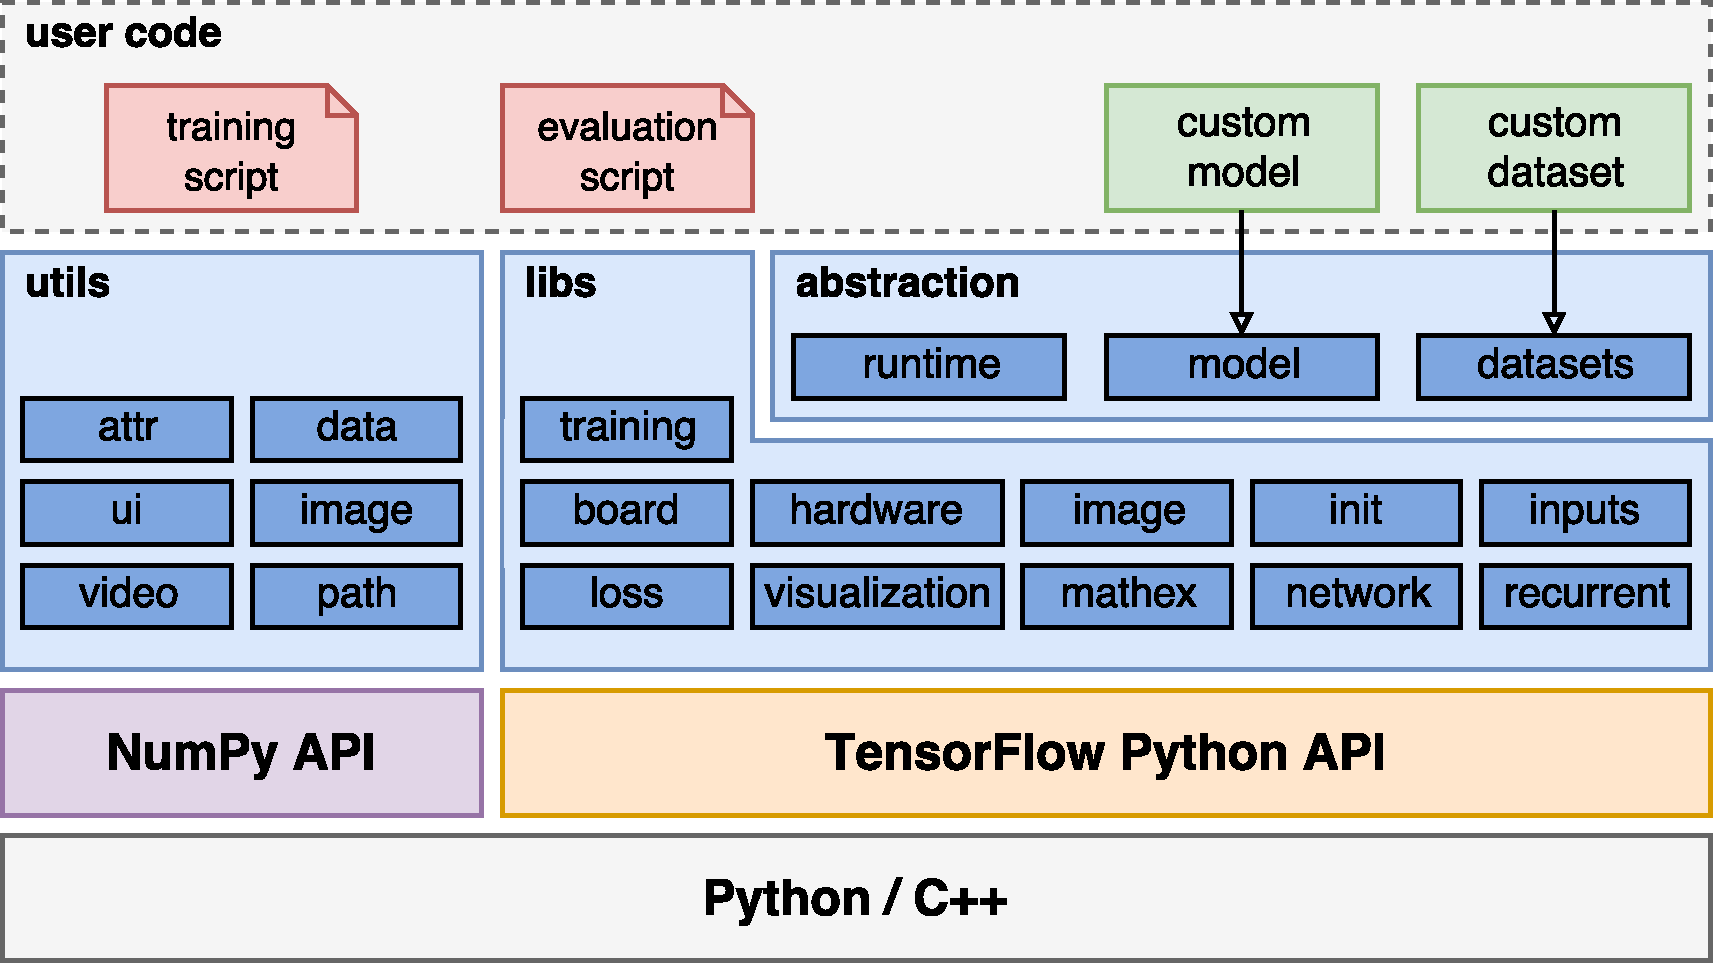
\includegraphics[width=0.8\linewidth]{figures/tensorlight_v3.pdf} 
	\caption[TensorLight Framework Architecture]{Architecture diagram of the TensorLight framework and its modules. The user program can take advantage of the provided abstraction layer, but also use the library and utility functions standalone.} \label{fig:tl_arch}
\end{figure}

The user program can either exploit the high-level library and the provided utility functions for his existing projects, or take advantage from TensorLight's abstraction layes while creating new deep learning applications. The latter enables to radically reduce the amount of code that has to be written for training or evaluating the model. This is realized by encapsulating the lifecycle of TensorFlow's session, graph, summary-writer or checkpoint-saver, as well as the entire training or evaluation loop within a \textit{runtime module}.


\subsection{Example}

This short example of a convolutional autoencoder, which reconstructs the entire input sequence of Moving MNIST, emphasizes the simplicity of deep learning applications implemented with TensorLight. At first, the model has to be defined. This is realized by implementing a class that derives from \texttt{tl.model.AbstractModel}. This class provides a standard interface to define the graph structure, the loss layer, as well as how this model has to be evaluated by the framework. The example's model implementation can be found in Figure \ref{code:model} in the appendix. In this case, the model is trained using binary cross-entropy. Moreover, image similarity metrics like PSNR, sharpness difference and SSIM are going be calculated and visualized in TensorBoard for every validation iteration in addition to the error value of the objective function.

\subsubsection*{Training}

The program code of an entire training process is depicted in Figure \ref{code:runtime_train}. Within the context of a runtime, the model, optimizer and datasets are registered with its parameters. Each runtime and dataset instance has a path-parameter in order to specify the root directory of the training outputs and meta files, as well as to reuse downloaded and preprocessed files across multiple processes. Afterwards, the computation graph is built and the training loop is started for \num{100} epochs. Since the example tries to reconstruct the inputs, one can set \texttt{autoencoder=True} in order to redirect the target pipeline of the dataset to the input data. Additionally, each batch of size \num{256} is distributed across two GPUs to speed up training.

\begin{figure}[htpb]
  \lstinputlisting[language=PythonEx,lastline=12]{code/runtime_train.py}
  \caption[Code: Training with TensorLight]{Example code for training a model with TensorLight. A convolutional autoencoder is trained on \textit{/gpu:0} and \textit{/gpu:1} for \num{100} epochs in order reconstruct Moving MNIST image sequences. It uses Adam optimizer with a low exponential learning rate decay.}
  \label{code:runtime_train}
\end{figure}

When the training is complete, the runtime is ready to do inference or testing on the model. In case the model's performance is still unsatisfactory, it is possible to continue the previous training for a few steps more. In addition, the framework allows to register a validation callback in order to perform specific functionality after every validation process. In this case, a GIF animation is generated that compares the ground truth with its reconstruction of a randomly generated sequence from the validation set. This is illustrated in Figure \ref{code:runtime_hook}.

\begin{figure}[htpb]
  \lstinputlisting[language=PythonEx,firstline=13,firstnumber=13]{code/runtime_train.py}
  \caption[Code: Continuing Training and Validation Hooks in TensorLight]{Code snippet that continues the previous training for another \num{10000} steps. Additionally, a validation hook is registered to write a GIF animation after every validation.}
  \label{code:runtime_hook}
\end{figure}


\subsubsection*{Evaluation}

After the whole training process is complete, the model is ready to get evaluated on the test set. Therefore, model and test dataset instances are created and registered to a new runtime object. When building the model, the last checkpoint file and the model's hyperparameter-meta file can be loaded in order to rebuild the graph with the identical weights and model configuration. Last but not least, the testing process can get started, as depicted in line 7 of Figure \ref{code:runtime_eval}.

\begin{figure}[htpb]
  \lstinputlisting[language=PythonEx]{code/runtime_eval.py}
  \caption[Code: Evaluation with TensorLight]{Code sample for testing a model on a single device in TensorLight. Before, it restores the checkpoint file containing all weights, as well as the model's hyperparameters of the previous training.}\label{code:runtime_eval}
\end{figure}
